% !TEX TS-program = pdflatex
% !TEX encoding = UTF-8 Unicode

\documentclass{beamer}
\usepackage[czech]{babel}
\usepackage[utf8]{inputenc}
\usepackage{times}
\usepackage[T1]{fontenc}
\usepackage{verbatim}
\usepackage{listings}
\usepackage{xcolor}

\mode<presentation>
{
	\usetheme{antibes}
	\usecolortheme{orchid}
}

\setbeamertemplate{navigation symbols}{}

\definecolor{cmtgreen}{RGB}{0,192,0}

\begin{document}

\title{C++; delete Java;}
\subtitle{Část 3: Výjimky}
\author{Kennny}
\date{srpen 2017}

\frame{\titlepage}

\lstset{language=C++,
        basicstyle=\ttfamily,
        keywordstyle=\color{blue}\ttfamily,
        stringstyle=\color{red}\ttfamily,
        commentstyle=\color{cmtgreen}\ttfamily,
        morecomment=[l][\color{magenta}]{\#}
}

\newenvironment{xframe}[1][]
  {\begin{frame}[fragile,environment=xframe,#1]}
  {\end{frame}}

\begin{comment}
\begin{xframe}{tttt}
	\begin{itemize}
		\item
	\end{itemize}
\end{xframe}
\end{comment}



\section{Výjimky}
\subsection{Princip}



\begin{xframe}{Výjimka}
	\begin{itemize}
		\item v C++ je výjimka pouze mechanismus
		\item neváže se na konkrétní datový typ
		\item syntaxe podobná jako jinde, pouze s menšími úpravami
\begin{lstlisting}[basicstyle=\fontsize{8}{9}\selectfont\ttfamily]
try
{
    throw std::overflow_error("Preteceni");
}
catch (std::invalid_argument& e)
{
    //
}
catch (...)
{
    //
}
\end{lstlisting}
	\end{itemize}
\end{xframe}

\begin{xframe}{Výjimka}
	\begin{itemize}
		\item instance se vytvoří ve scope příslušného \texttt{catch} bloku
		\item pomocí \texttt{throw} vyhazujeme staticky alokované (throw by-value)
		\item pomocí \texttt{catch} je lepší odchytávat reference (catch by-reference)
			\begin{itemize}
				\item odchytávání hodnotou nezohledňuje polymorfismus
			\end{itemize}
		\item za \texttt{throw} může být libovolný datový typ
\begin{lstlisting}[basicstyle=\fontsize{8}{9}\selectfont\ttfamily]
try
{
    throw int(5);
}
catch (int& e)
{
    //
}
\end{lstlisting}
	\end{itemize}
\end{xframe}


\begin{xframe}{Standardní výjimky}
	\begin{itemize}
		\item STL obsahuje standardní výjimky
		\item ty používají všechny STL třídy, je možné (někdy i vhodné) je používat také
		\item popřípadě si oddědit vlastní
		\item specifikátor \texttt{throw()} specifikující typy, co metoda může vyhodit
			\begin{itemize}
				\item nedoporučuje se
				\item maximálně čistý \texttt{throw()} kde víme, že nikdy výjimka nevznikne
			\end{itemize}
	\end{itemize}
\end{xframe}

\begin{xframe}{std::exception}
	\begin{figure}[ht]
		\centering
		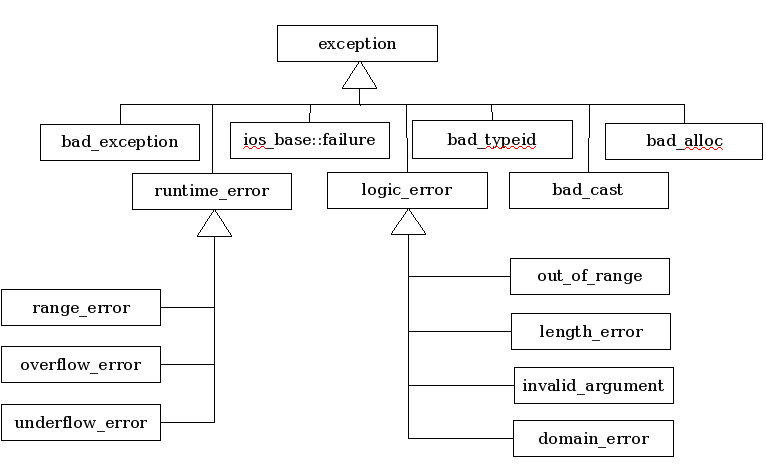
\includegraphics[width=0.9\textwidth]{std_exceptions.png}
		\caption{Hierarchie základních STL výjimek}
	\end{figure}
\end{xframe}

\begin{xframe}{std::exception}
	\begin{itemize}
		\item base class pro všechny STL výjimky
		\item konstruktor a metoda \texttt{what}, která vrací řetězec s chybou
		\item jedná se ale o kostru - konstruktor bez parametru, \texttt{what} vrací prázdný řetězec
		\item potomci definují vlastní konstruktor a přepisují \texttt{what}
	\end{itemize}
\end{xframe}

\begin{xframe}{Vlastní výjimková třída}
\begin{lstlisting}[basicstyle=\fontsize{8}{9}\selectfont\ttfamily]
class CustomException : public std::exception
{
    public:
        CustomException(std::string& what)
        {
            m_what = "Custom exception: " + what;
        }

        const char* what() const throw()
        {
            return m_what.c_str();
        };
    private:
        std::string m_what;
};
\end{lstlisting}
\end{xframe}

\begin{xframe}{Poznámky}
	\begin{itemize}
		\item výjimku lze "odhodit"~v catch bloku do vyšších handlerů
\begin{lstlisting}[basicstyle=\fontsize{8}{9}\selectfont\ttfamily]
catch (std::exception& e)
{
    throw;   // ta sama instance
    throw e; // vytvori novou instanci kopii
}
\end{lstlisting}
		\item odchycení všech výjimek (resp. zbytku): syntaxe třech teček
\begin{lstlisting}[basicstyle=\fontsize{8}{9}\selectfont\ttfamily]
catch (...)
{
    // handler
}
\end{lstlisting}
	\end{itemize}
\end{xframe}

\begin{xframe}{Praktiky}
	\begin{itemize}
		\item využít existující STL výjimku nebo oddědit vlastní výjimku od \texttt{std::exception}
		\item nepoužívat výjimky pokud to není nutné - nestandardní flow
		\item odchytávat pokud možno co nejspecifičtější výjimky (znalost situace), ale zbytečně neriskovat
		\item \emph{throw by value, catch by reference}; nealokovat dynamicky
	\end{itemize}
\end{xframe}


\begin{xframe}{Příklad}
	\begin{itemize}
		\item Prostor pro příklad 03\_a\_exceptions
	\end{itemize}
\end{xframe}




\begin{xframe}{Konec 3. části}
\texttt{exit(0);}
\end{xframe}




\end{document}




